\documentclass[10pt,twocolumn]{article}

% ── Packages ──────────────────────────────────────────────────────────────────
\usepackage{fourier}

\usepackage[margin=1in]{geometry}
\setlength{\columnsep}{20pt}
\usepackage{parskip}
\usepackage{amsmath,amssymb,amsthm}
\usepackage{graphicx}
\usepackage{booktabs}
\usepackage{hyperref}
\usepackage{xcolor}
\usepackage{microtype}
\usepackage{enumitem}
\usepackage{caption}
\captionsetup{font=small, labelfont=bf}
\usepackage{subcaption}
\usepackage{multirow}
\usepackage{array}
\usepackage{natbib}
\usepackage{tikz}
\usetikzlibrary{arrows.meta,positioning,fit,backgrounds,calc}

% ── Macros ────────────────────────────────────────────────────────────────────
\newcommand{\vit}{ViT}
\newcommand{\cifar}{CIFAR-10}
\newcommand{\pp}{\,pp}   % percentage points
\newcommand{\methodA}{Frozen Patch-Whitening}
\newcommand{\methodB}{Dirac Initialisation}
\newcommand{\methodC}{ScaleBias + Lookahead}
\newcommand{\methodD}{Alternating Flip}

\hypersetup{
    colorlinks=true,
    linkcolor=blue!60!black,
    citecolor=blue!60!black,
    urlcolor=blue!60!black,
}

% ── Title ─────────────────────────────────────────────────────────────────────
\title{%
    \textbf{Do CNN Speed-Up Tricks Transfer to Transformers?}\\
    \large Evaluating Fast-Training Techniques on Vision Transformers for {\cifar}
}

\author{
    \textit{COMP-4471: Deep Learning in Computer Vision --- Course Project}\\[2pt]
    The Hong Kong University of Science and Technology
}

\date{}

% ══════════════════════════════════════════════════════════════════════════════
\begin{document}
\maketitle

% ── Abstract ──────────────────────────────────────────────────────────────────
\begin{abstract}
    Recent work by \citet{garg2024cifar10} demonstrated that a carefully engineered CNN can reach $94\%$ accuracy on CIFAR-10 in 3.29 seconds on a single GPU, using four training tricks: frozen patch-whitening initialisation, Dirac (identity) initialisation, a ScaleBias output layer with the Lookahead optimiser, and alternating horizontal flip.
    We ask whether these tricks transfer to transformer architectures.
    We train a small Vision Transformer (ViT, $\sim$4M parameters) on CIFAR-10 under two regimes: a weak recipe (100 epochs, basic augmentation, $61.7\%$ baseline) and a strong recipe (300 epochs, RandAugment, Mixup/CutMix, DropPath, $81.4\%$ baseline).
    Under the weak recipe, representation-quality tricks (whitening, alternating flip) transfer positively ($+1.3$\pp{} and $+0.8$\pp{}) while architecture-specific tricks (Dirac init, ScaleBias+Lookahead) are harmful ($-7.9$\pp{} and $-16.0$\pp{}).
    Under the strong recipe the picture partially reverses: whitening and alternating flip become slightly negative ($-4.4$\pp{} and $-0.8$\pp{}) while soft Dirac init ($\alpha=0.3$) turns marginally positive ($+0.4$\pp{}).
    We attribute the whitening reversal to a frozen-embedding/augmentation conflict: whitened filters computed from clean images are mismatched to the heavily transformed inputs produced by Mixup and CutMix.
    These findings reveal that the transferability of CNN training tricks depends critically on the training recipe, not just on architectural compatibility.
\end{abstract}

% ── 1. Introduction ───────────────────────────────────────────────────────────
\section{Introduction}\label{sec:intro}

The dominant paradigm for fast and accurate image classification has shifted from hand-crafted convolutional networks to Vision Transformers \citep{dosovitskiy2021vit}. Yet many practical training recipes are still rooted in CNN-era knowledge: specific weight initialisations, output-layer scaling, and data-augmentation strategies devised with convolution in mind.

\citet{garg2024cifar10} packaged four such techniques into a record-breaking CIFAR-10 run -- $94\%$ accuracy in under 3.3 seconds on a single RTX 4090. Their approach raises a natural question: \emph{how much of the speed and accuracy gain comes from properties specific to convolutional inductive bias, and how much is transferable to other architectures?}

We answer this empirically for the Vision Transformer. Our contributions are:
\begin{enumerate}[leftmargin=*, itemsep=0pt]
    \item Two ViT baselines on CIFAR-10: a weak recipe ($61.7\%$, 100 epochs) and a strong recipe ($81.4\%$, 300 epochs with RandAugment, Mixup/CutMix, DropPath).
    \item Per-trick ablations under both recipes, isolating each technique's effect.
    \item An analysis of why the same trick can help under one recipe and hurt under another, with particular attention to the frozen-whitening/augmentation conflict.
\end{enumerate}

% ── 2. Background ─────────────────────────────────────────────────────────────
\section{Background}\label{sec:background}

\subsection{Fast CNN Training on CIFAR-10}
\citet{garg2024cifar10} build on the DAWNBench lineage \citep{coleman2017dawnbench} and the earlier ``how to train your ResNet'' series. Their key observation is that several operations -- the initial patch embedding, the output scaling, the data augmentation schedule -- can be made more efficient or more principled without degrading accuracy. The four techniques they employ are described in Section~\ref{sec:methods}.

\subsection{Vision Transformers}
A Vision Transformer \citep{dosovitskiy2021vit} splits an image into non-overlapping patches, linearly projects each patch to an embedding vector, appends a learnable \texttt{[CLS]} token, adds positional embeddings, and passes the sequence through a stack of multi-head self-attention and MLP blocks. The classification head operates on the \texttt{[CLS]} output.

ViT was designed for large-scale pretraining; adapting it to small datasets like CIFAR-10 requires smaller models and stronger regularisation. We follow the ``ViT-Tiny'' spirit \citep{touvron2021deit}: patch size~4, embedding dimension 192, depth~9, 4 attention heads, $\sim$4M parameters.

% ── 3. Methods ────────────────────────────────────────────────────────────────
\section{Methods}\label{sec:methods}

\subsection{Model Architecture}\label{sec:arch}
\begin{figure*}[t]
    \centering
    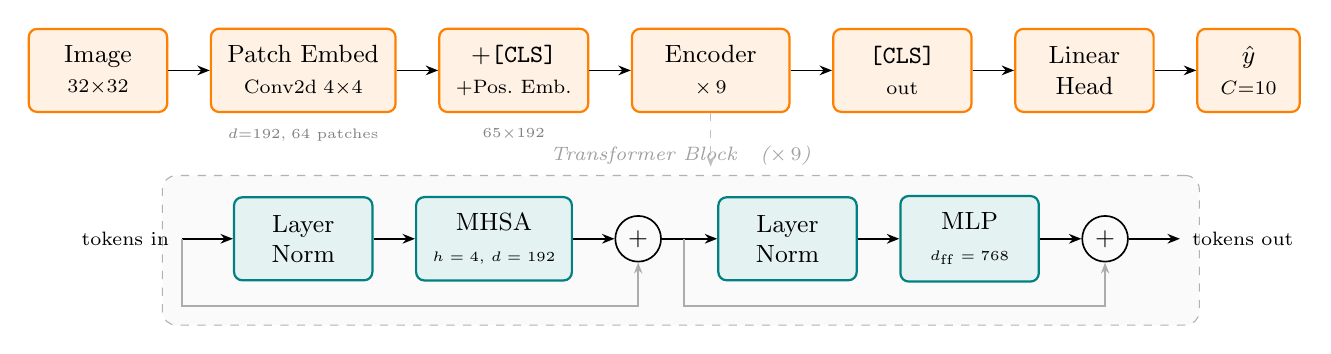
\begin{tikzpicture}[node distance = 0.5cm and 0.55cm,
        % Main pipeline boxes
        M/.style = {
                draw=orange, fill=orange!10, thick,
                rounded corners=3pt,
                minimum width=50pt, minimum height=30pt,
                inner sep=6pt,
                align=center, font=\small
            },
        % Transformer block boxes
        B/.style = {
                draw=teal, fill=teal!10, thick,
                rounded corners=3pt,
                minimum width=50pt, minimum height=30pt,
                inner sep=6pt,
                align=center, font=\small
            },
        circ/.style = {circle, draw, semithick, inner sep=2.5pt, font=\small},
        arr/.style  = {-{Stealth[length=4.5pt,width=3.5pt]}, semithick},
        skip/.style = {-{Stealth[length=4pt,width=3pt]}, semithick, gray!65},
        ]

        %------------------------------------------------------------------
        % Top row: overall ViT pipeline (left to right)
        %------------------------------------------------------------------
        \node[M] (img)   {Image\\{\scriptsize$32{\times}32$}};
        \node[M, right=15pt of img] (pemb) {Patch Embed\\{\scriptsize Conv2d\;$4{\times}4$}};
        \node[M, right=15pt of pemb] (addcls) {$+$\texttt{[CLS]}\\{\scriptsize +Pos.\ Emb.}};
        \node[M, right=15pt of addcls, minimum width=2.0cm] (encblk) {Encoder\\{\scriptsize$\times\,9$}};
        \node[M, right=15pt of encblk] (clsout) {\texttt{[CLS]}\\{\scriptsize out}};
        \node[M, right=15pt of clsout] (linH) {Linear\\Head};
        \node[M, right=15pt of linH, minimum width=1.3cm] (pred) {$\hat{y}$\\{\scriptsize$C{=}10$}};

        \foreach \a/\b in {img/pemb, pemb/addcls, addcls/encblk,
                encblk/clsout, clsout/linH, linH/pred}
        \draw[arr] (\a) -- (\b);

        % Subscript annotations
        \node[font=\tiny, gray, below=2pt of pemb]   {$d{=}192$,\;64 patches};
        \node[font=\tiny, gray, below=2pt of addcls] {$65{\times}192$};

        %------------------------------------------------------------------
        % Bottom row: one transformer block detail (left to right)
        %------------------------------------------------------------------
        \node[B,    below=30pt of pemb ] (bln1)  {Layer\\Norm};
        \node[B,    right=15pt of bln1 ] (bmha)  {MHSA\\{\tiny$h=4$, $d=192$}};
        \node[circ, right=15pt of bmha ] (badd1) {$+$};
        \node[B,    right=20pt of badd1] (bln2)  {Layer\\Norm};
        \node[B,    right=15pt of bln2 ] (bmlp)  {MLP\\{\tiny$d_\mathrm{ff}=768$}};
        \node[circ, right=15pt of bmlp ] (badd2) {$+$};

        % tokens in / out markers
        \coordinate (bin)  at ([xshift=-0.65cm] bln1.west);
        \coordinate (bout) at ([xshift= 0.65cm] badd2.east);
        \node[font=\scriptsize, left=1pt of bin,  anchor=east]  {tokens in};
        \node[font=\scriptsize, right=1pt of bout, anchor=west] {tokens out};

        % mid-point between badd1 and bln2 for skip-2
        \coordinate (mid12) at ($(badd1.east)!0.4!(bln2.west)$);

        % main horizontal arrows
        \draw[arr] (bin)   -- (bln1);
        \draw[arr] (bln1)  -- (bmha);
        \draw[arr] (bmha)  -- (badd1);
        \draw[arr] (badd1) -- (bln2);
        \draw[arr] (bln2)  -- (bmlp);
        \draw[arr] (bmlp)  -- (badd2);
        \draw[arr] (badd2) -- (bout);

        % skip 1: bin -> badd1  (U-turn below, wider)
        \coordinate (s1a) at ([yshift=-0.85cm] bin);
        \coordinate (s1b) at (s1a -| badd1.south);
        \draw[skip] (bin)   -- (s1a) -- (s1b) -- (badd1.south);

        % skip 2: mid12 -> badd2  (U-turn below, narrower)
        \coordinate (s2a) at ([yshift=-0.85cm] mid12);
        \coordinate (s2b) at (s2a -| badd2.south);
        \draw[skip] (mid12) -- (s2a) -- (s2b) -- (badd2.south);

        % dashed bounding box around the block
        \begin{scope}[on background layer]
            \node[draw=gray!60, dashed, rounded corners=5pt, fill=gray!4,
            fit=(bin)(bln1)(bmha)(badd1)(bln2)(bmlp)(badd2)(bout)(s1a)(s1b)(s2a)(s2b),
            inner sep=7pt,
            label={[font=\scriptsize\itshape, gray!75]
            above:{Transformer Block\quad($\times\,9$)}}] (blkframe) {};
        \end{scope}

        % dashed leader from encblk down to blkframe
        \draw[dashed, gray!50, -{Stealth[length=4pt]}, shorten >=3pt]
        (encblk.south) -- (encblk.south |- blkframe.north);

    \end{tikzpicture}
    \caption{\textbf{Top}: overall ViT pipeline (left to right).
        The $32{\times}32$ input is split into $4{\times}4$ patches and projected to
        dimension~192.  A learnable \texttt{[CLS]} token is prepended and positional
        embeddings are added (65 tokens).  Nine Transformer Encoder blocks process
        the sequence; the \texttt{[CLS]} output feeds a linear classifier.
        \textbf{Bottom}: detail of one encoder block (Pre-LN, left to right).
        Each sub-layer (MHSA and MLP) is preceded by Layer Norm and wrapped in a
        residual (skip) connection shown in grey.}
    \label{fig:architecture}
\end{figure*}

All experiments use the same ViT; configuration details are given in Table~\ref{tab:vit-config}. Figure~\ref{fig:architecture} illustrates the overall pipeline and one encoder block.

The patch embedding is a $4\times4$ Conv2d layer, exposing its weights for the
initialisation experiments. The default classifier is a linear layer on the \texttt{[CLS]} token.

\subsection{Training Setup}\label{sec:training}

\begin{table*}[ht]
    \centering
    \begin{minipage}[t]{0.36\linewidth}
        \vspace{0pt}
        \centering
        \begin{tabular}{ll}
            \toprule
            Hyperparameter  & Value                   \\
            \midrule
            Image size      & $32\times32$            \\
            Patch size      & $4\times4$ (64 patches) \\
            Embedding dim   & 192                     \\
            Depth           & 9 blocks                \\
            Attention heads & 4                       \\
            MLP ratio       & 4.0                     \\
            Dropout         & 0.1                     \\
            Parameters      & 4{,}028{,}170           \\
            \bottomrule
        \end{tabular}
        \captionof{table}{ViT configuration used for all experiments.}
        \label{tab:vit-config}
    \end{minipage}
    \hfill
    \begin{minipage}[t]{0.58\linewidth}
        \vspace{0pt}
        \centering
        \begin{tabular}{lll}
            \toprule
            Hyperparameter  & Weak recipe      & Strong recipe                   \\
            \midrule
            Epochs          & $100$            & $300$                           \\
            Batch size      & $256$            & $256$                           \\
            Optimiser       & AdamW            & AdamW                           \\
            Peak LR         & $3\times10^{-4}$ & $1\times10^{-3}$                \\
            LR schedule     & OneCycleLR       & Cosine + 5\% warmup             \\
            Weight decay    & $0.05$           & $0.05$                          \\
            DropPath rate   & ---              & $0.1$ (linear)                  \\
            Augmentation    & Crop + flip      & Crop + flip + RandAugment       \\
            Mixup/CutMix    & ---              & $\alpha=0.8$ / $\alpha=1.0$ \\
            Label smoothing & $0.1$            & $0.1$                           \\
            AMP             & \texttt{float16} & \texttt{float16}                \\
            \bottomrule
        \end{tabular}
        \captionof{table}{Training setup. All experiments within each recipe share these hyperparameters.}
        \label{tab:training-setup}
    \end{minipage}
\end{table*}

All experiments use one of two recipes, both detailed in Table~\ref{tab:training-setup}. The \textbf{weak recipe} (100 epochs, basic augmentation) serves as a controlled environment for isolating per-trick effects. The \textbf{strong recipe} (300 epochs, RandAugment, Mixup/CutMix, DropPath) reflects a realistic, state-of-the-art ViT training setup and tests whether the tricks transfer at a higher accuracy floor ($81.4\%$ vs.\ $61.7\%$).

The strong recipe adds three components absent from the weak recipe:
\begin{itemize}[leftmargin=*]
    \item \textbf{DropPath} (stochastic depth, linearly scaled $0 \to 0.1$ across the 9 blocks): regularises residual paths in deep transformers.
    \item \textbf{RandAugment} ($n=2$, $m=9$): random colour and geometric operations applied after crop and flip.
    \item \textbf{Mixup / CutMix} ($\alpha=0.8$ / $\alpha=1.0$, each $50\%$ probability per batch): soft-label interpolation that is the primary diversity source for ViTs on small datasets.
\end{itemize}

\subsection{Frozen Patch-Whitening Initialisation}\label{sec:whitening}

In the source CNN, the first convolution is initialised with whitened eigenvectors of the training-set patch covariance and then frozen. Formally, let $\mathbf{P} \in \mathbb{R}^{N \times D}$ be the matrix of all $(C \times H \times W)$-dimensional patches. We compute $\mathbf{C} = \mathbf{P}^\mathrm{T} \mathbf{P} / N$ and its eigendecomposition $\mathbf{C} = \mathbf{V} \boldsymbol{\Lambda} \mathbf{V}^\mathrm{T}$. The whitening filters are $\mathbf{V} {(\boldsymbol{\Lambda} + \varepsilon \mathbf{I})}^{-1/2}$, and we initialise the Conv2d weights in the patch embedding with both positive and negative copies of the leading eigenvectors
\begin{equation}
    W_k = -W_{k+D} = \frac{\mathbf{v}_k}{\sqrt{\lambda_k + \varepsilon}},
    \quad k = 1, \dots, D,
\end{equation}
where $D = C \times H \times W = 3\times4\times4 = 48$ and the embedding dimension
is 192, so the first 96 channels are filled and the remaining 96 retain their
default (He) initialisation.
The embedding weights are frozen (\texttt{requires\_grad=False}) for the entire
training run.

\subsection{Dirac/Identity Initialisation}\label{sec:dirac}
The source CNN initialises its Conv layers so that the first $C_\text{in}$
output channels compute the identity (Dirac delta) map.
For a $1\times1$ convolution this reduces to $W = \mathbf{I}$.

We adapt this to the attention projections.
The combined QKV weight $\mathbf{W}_{QKV} \in \mathbb{R}^{3D \times D}$ is
partitioned into three $D\times D$ blocks, each set to $\mathbf{I}_D$.
The output projection $\mathbf{W}_O \in \mathbb{R}^{D\times D}$ is also set to
$\mathbf{I}_D$.
All associated biases are zeroed.

\subsection{ScaleBias + Lookahead}\label{sec:scalebias}
The source CNN appends a \texttt{Scale(1/9)} module after the final global
pooling to stabilise output magnitude.
We generalise this to a learnable per-feature affine transform
$y_i = s_i x_i + b_i$ (ScaleBias), initialised with $s_i = 1/9$, $b_i = 0$,
replacing the standard linear head.

The Lookahead optimiser \citep{zhang2019lookahead} maintains a set of \emph{slow weights} $\phi$ alongside the fast weights $\theta$ of any inner optimiser
\begin{equation}
    \phi_{t+k} \gets \phi_t + \alpha \left( \theta_{t+k} - \phi_t \right), \quad
    \theta \gets \phi_{t+k}
\end{equation}
with $k=6$, $\alpha=0.5$. We wrap AdamW with Lookahead as in the original paper.

\subsection{Alternating Flip}\label{sec:altflip}
Standard random horizontal flip applies a Bernoulli($p=0.5$) per sample,
introducing batch-level variance in flip counts.
Alternating flip instead deterministically flips every odd-indexed sample in the
dataset, guaranteeing exactly 50\% flipped samples in every epoch.
The only change is replacing \texttt{random.random() > 0.5} with
\texttt{(idx \% 2 == 1)}.

\begin{figure*}[t]
    \centering
    \begin{subfigure}[t]{0.48\linewidth}
        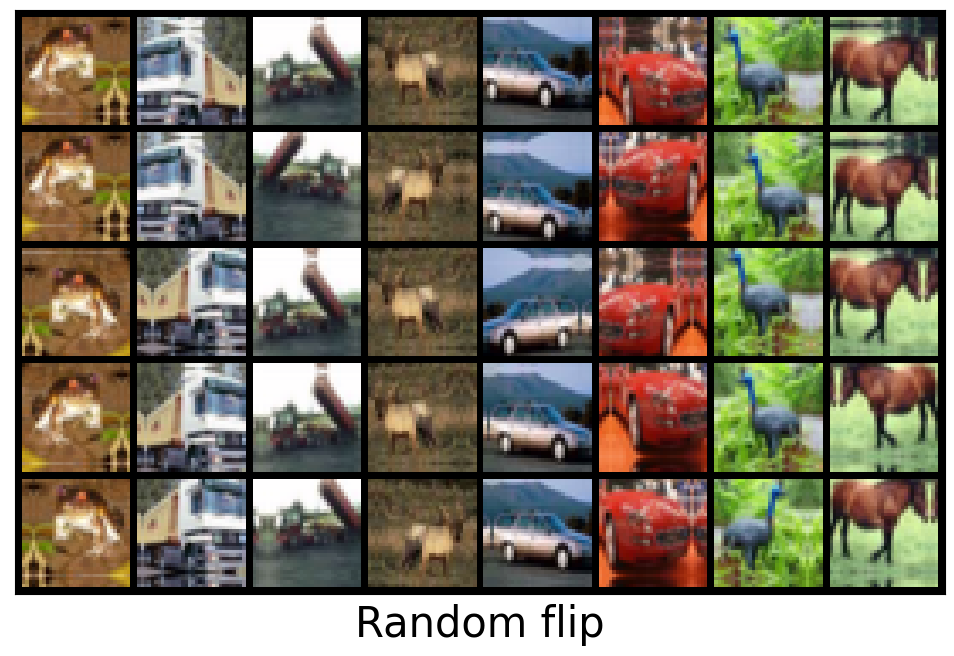
\includegraphics[width=\linewidth]{figures/random_flip.png}
        \caption{Random flip: each sample is flipped independently with
            $p{=}0.5$, so the number of flipped images varies between
            batches.}
        \label{fig:random-flip}
    \end{subfigure}
    \hfill
    \begin{subfigure}[t]{0.48\linewidth}
        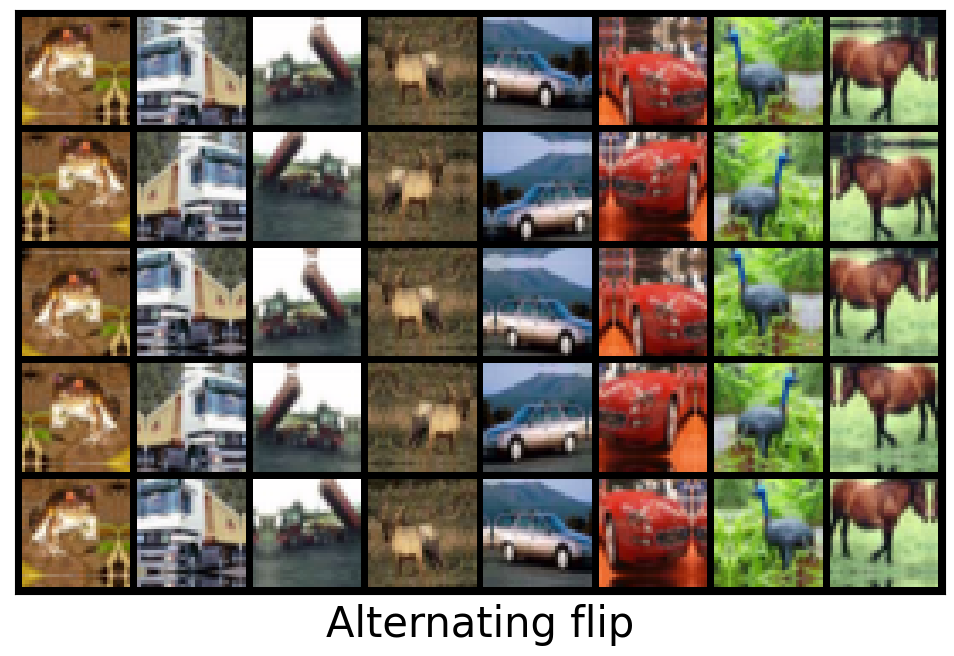
\includegraphics[width=\linewidth]{figures/alternating_flip.png}
        \caption{Alternating flip: every odd-indexed sample is flipped,
            guaranteeing exactly 50\% flipped images in every epoch and
            eliminating batch-level flip-count variance.}
        \label{fig:alt-flip}
    \end{subfigure}
    \caption{Comparison of random flip (left) and alternating flip (right)
        over five consecutive epochs on the same eight CIFAR-10 images.
        Columns are images; rows are epochs.  Random flip produces
        inconsistent flip patterns across epochs, whereas alternating flip
        applies a fixed odd/even assignment that repeats identically every
        epoch.}
    \label{fig:flip-comparison}
\end{figure*}

\subsection{All Methods Combined}
We also run one experiment that applies all four tricks simultaneously, using
the same whitened and frozen patch embedding, Dirac-initialised attention,
ScaleBias head, Lookahead optimiser, and alternating flip.

% ── 4. Experiments ────────────────────────────────────────────────────────────
\section{Experiments}\label{sec:experiments}

\subsection{Setup}
Experiments run on a single NVIDIA RTX 4090 (24\,GB VRAM) per run, with four
runs in parallel across four available GPUs.
All results use the checkpoint with the highest validation accuracy.
We report accuracy on the fixed CIFAR-10 test set of 10{,}000 images.

\subsection{Results}
Table~\ref{tab:results} summarises the final test accuracy under both recipes.
Figure~\ref{fig:curves} shows the validation curves over 300 epochs (strong recipe).

\begin{table*}[ht]
    \centering
    \begin{tabular}{lrrrr}
        \toprule
        \multirow{2}{*}{Experiment}
                                            & \multicolumn{2}{c}{Weak recipe (100 ep, 61.68\% base)}
                                            & \multicolumn{2}{c}{Strong recipe (300 ep, 81.42\% base)}                                                   \\
        \cmidrule(lr){2-3}\cmidrule(lr){4-5}
                                            & Test Acc.                                                & $\Delta$      & Test Acc.        & $\Delta$     \\
        \midrule
        Baseline                            & 61.68\%                                                  & ---           & 81.42\%          & ---          \\
        \midrule
        + \methodA{}                        & \textbf{62.99\%}                                         & $+$1.31\pp{}  & 77.03\%          & $-$4.39\pp{} \\
        + \methodD{}                        & 62.48\%                                                  & $+$0.80\pp{}  & 80.60\%          & $-$0.82\pp{} \\
        + \methodB{} (full)                 & 53.78\%                                                  & $-$7.90\pp{}  & 79.20\%          & $-$2.22\pp{} \\
        + \methodB{} (soft, $\alpha{=}0.3$) & 60.52\%                                                  & $-$1.16\pp{}  & \textbf{81.83\%} & $+$0.41\pp{} \\
        + \methodC{}                        & 45.71\%                                                  & $-$15.97\pp{} & 76.39\%          & $-$5.03\pp{} \\
        \midrule
        All methods                         & 38.05\%                                                  & $-$23.63\pp{} & 71.74\%          & $-$9.68\pp{} \\
        \bottomrule
    \end{tabular}
    \caption{Test accuracy (\%) under the weak recipe (100 epochs, basic augmentation) and
        the strong recipe (300 epochs, RandAugment + Mixup/CutMix + DropPath).
        $\Delta$ is relative to the corresponding baseline.
        The strong-recipe \methodC{} uses scale$=$1.0 and cosine LR.}
    \label{tab:results}
\end{table*}

\begin{figure*}[ht]
    \centering
    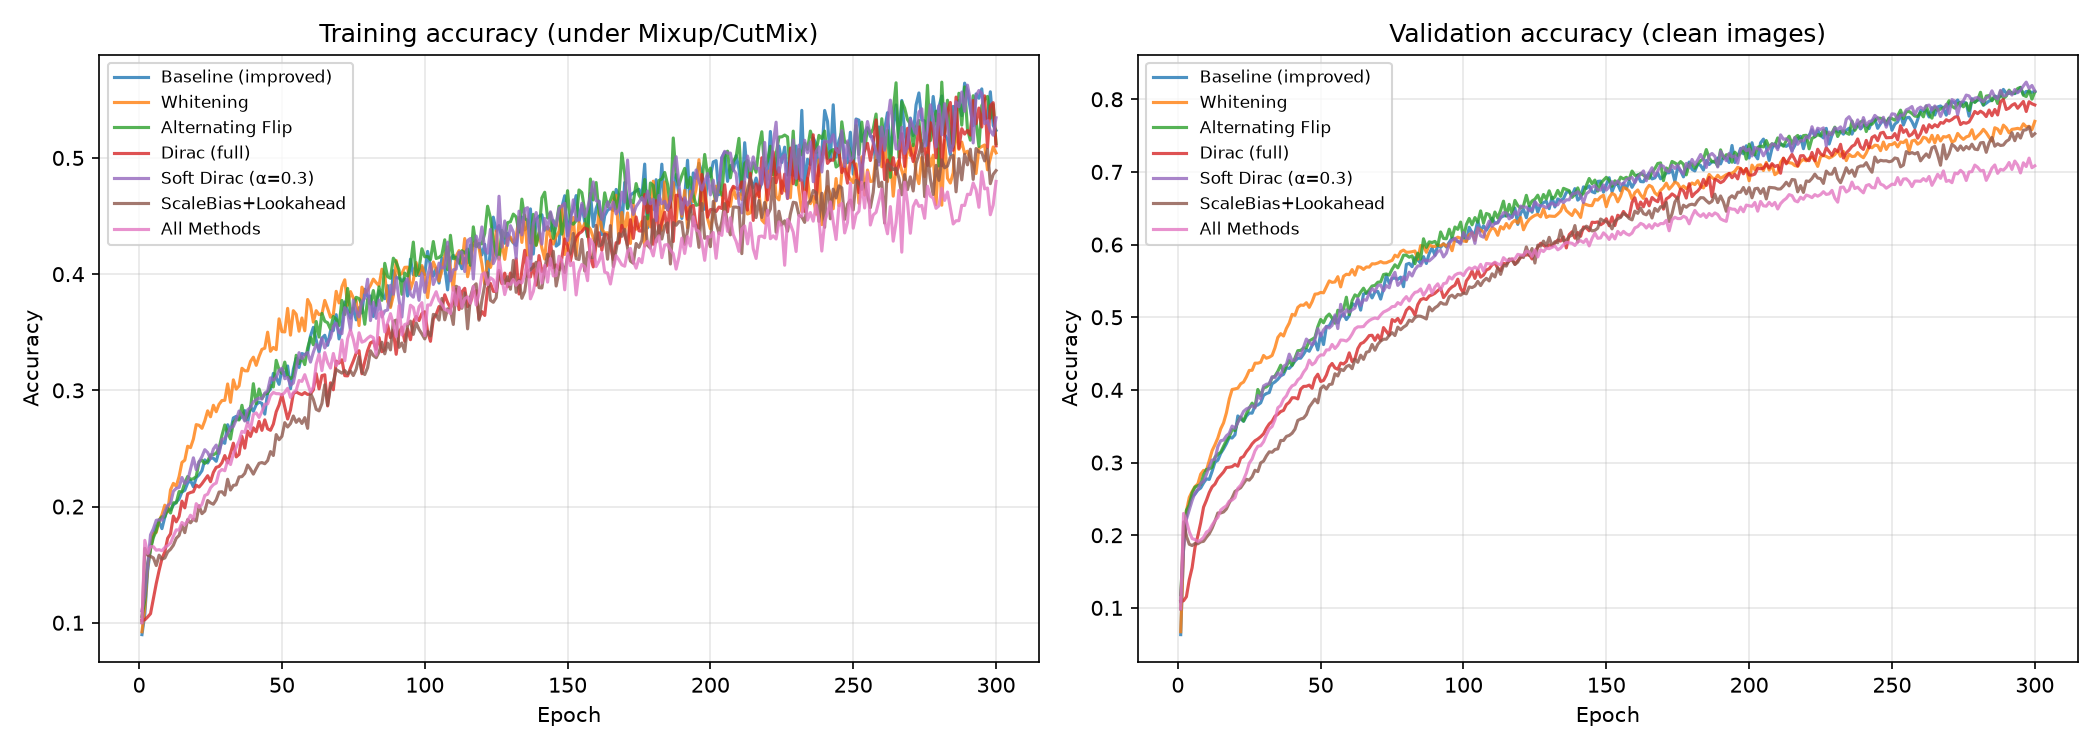
\includegraphics[width=\linewidth]{../experiments/comparison_v3.png}
    \caption{Validation accuracy over 300 epochs (strong recipe).
        Soft Dirac ($\alpha{=}0.3$) and Alternating Flip track closely with the
        baseline; Whitening, ScaleBias+Lookahead, and All Methods fall behind.}
    \label{fig:curves}
\end{figure*}

Table~\ref{tab:epochs} traces the validation accuracy at selected epochs (strong recipe),
revealing \emph{how} the tricks affect convergence speed.

\begin{table}[ht]
    \centering
    \setlength{\tabcolsep}{4pt}
    \begin{tabular}{rcccccc}
        \toprule
        Epoch & Base          & Altflip       & White.        & Dirac & SB+LA & All  \\
        \midrule
        50    & 47.8          & 49.7          & \textbf{53.4} & 41.2  & 40.2  & 44.8 \\
        100   & 61.6          & 60.9          & \textbf{60.5} & 53.4  & 53.3  & 55.7 \\
        150   & 68.2          & \textbf{69.3} & 65.2          & 63.6  & 63.2  & 61.2 \\
        200   & 71.9          & \textbf{73.8} & 68.8          & 69.6  & 67.8  & 65.3 \\
        250   & 75.7          & \textbf{77.3} & 73.8          & 74.7  & 71.5  & 68.3 \\
        300   & \textbf{81.1} & 81.0          & 77.0          & 79.2  & 75.3  & 70.8 \\
        \bottomrule
    \end{tabular}
    \caption{Validation accuracy (\%) at selected epochs, strong recipe.
        Bold marks the highest per row.}
    \label{tab:epochs}
\end{table}


% ── 5. Analysis ───────────────────────────────────────────────────────────────
\section{Analysis}\label{sec:analysis}

\subsection{Why Whitening Flips Sign Across Recipes}\label{sec:whitening-analysis}
Patch whitening removes second-order correlations from the input token embeddings, providing a more isotropic feature space at initialisation.
Under the weak recipe this helps immediately: at epoch~1, whitening already achieves 30.7\% vs.\ the baseline's 28.3\%, and the gap holds to $+1.31$\pp{} at epoch 100 (Table~\ref{tab:results}).
The mechanism is architecture-agnostic---the covariance structure of local patches is a property of the data, not the model.

Under the strong recipe, however, whitening \emph{reverses}: $-4.39$\pp{} (77.03\%).
The cause is a \textbf{frozen-embedding / augmentation conflict}.
The whitened filters are eigenvectors of the patch covariance computed from \emph{clean} training images, and the embedding is frozen for the whole run.
Under the strong recipe, each input is first RandAugmented, then mixed with another image (Mixup) or cut-and-pasted (CutMix)---so the patch embedding never sees inputs whose statistics match the basis it was computed from.
A frozen basis that was optimal for clean patches is mismatched to heavily transformed ones, and because it is frozen it cannot adapt.
Under the weak recipe the only augmentation is crop+flip, which preserves patch covariance closely enough that the whitening basis stays useful.

Table~\ref{tab:epochs} confirms this reading: at epoch~50 whitening leads all methods (53.4\% vs.\ 47.8\% baseline), but the baseline overtakes it by epoch~150 and the gap widens through epoch~300.
The whitened model starts strong---better initial features---but plateaus earlier because its frozen patch embedding cannot track the representation drift that strong augmentation induces in the rest of the network.
This is the clearest demonstration in our results that a trick's effect is not a property of the trick alone but of the trick $\times$ recipe interaction.

\subsection{Why Alternating Flip Also Flips Sign}
Alternating flip replaces a stochastic 50\% flip with a deterministic one.
Under the weak recipe it helps marginally ($+0.80$\pp{}): reducing batch-level flip-count variance lowers gradient noise, which matters when the model sees little other augmentation.
Under the strong recipe it turns slightly negative ($-0.82$\pp{}).
With RandAugment and Mixup/CutMix already providing large per-sample diversity, the marginal variance reduction from deterministic flipping is swamped; meanwhile the loss of \emph{randomness} removes a mild regularisation effect, since a fixed flip pattern is easier for the model to memorise than a stochastic one.
The magnitude is small in both directions, confirming that flip strategy is a low-impact lever once stronger augmentation is present.

\subsection{Why Dirac Init Hurts, and Why Strong Augmentation Helps It}\label{sec:dirac-analysis}
In the source CNN, initialising a $k\times k$ convolution to the Dirac delta means the first $C$ output filters simply copy their input channels, akin to a near-identity residual path.
Applying the same logic to attention projections yields a pathological starting point.
With $\mathbf{W}_Q = \mathbf{W}_K = \mathbf{W}_V = \mathbf{I}$ and $\mathbf{W}_O = \mathbf{I}$, the attention output at initialisation is
\begin{equation}
    \operatorname{Attn} \!\left( X \right) =
    \operatorname{softmax} \!\left( \frac{ X X^\mathrm{T} }{ \sqrt{d} } \right) X,
\end{equation}
a diffuse uniform pattern in which every head computes the same transformation.
The model must first \emph{break the symmetry} before it can specialise.

Two observations support this diagnosis.
First, the gap shrinks from $-7.90$\pp{} (weak) to $-2.22$\pp{} (strong): strong augmentation supplies the diverse gradients needed to break the symmetry faster, so less training time is wasted.
Second, \textbf{soft} Dirac init---an interpolation $\mathbf{W} \leftarrow \alpha\mathbf{I} + (1-\alpha)\mathbf{W}_\text{rand}$ at $\alpha{=}0.3$---goes from $-1.16$\pp{} (weak) to $+0.41$\pp{} (strong), the only trick that is net-positive under the strong recipe.
A 30\% identity blend preserves enough random structure that the heads do not collapse, while still giving each a mild identity prior; combined with strong augmentation this becomes a small benefit rather than a cost.

\subsection{Why ScaleBias + Lookahead Hurts}\label{sec:sbl-analysis}
Two independent issues combine here.

\paragraph{ScaleBias scale initialisation.}
The ScaleBias head is initialised with $s_i = 1/9$.
Because the head output is $\hat{y} = \mathbf{W}_\text{head}(\mathbf{s} \odot \mathbf{x} + \mathbf{b})$, the effective gradient reaching the transformer body is scaled by $1/9 \approx 0.11\times$ relative to a standard linear head.
In the CNN, a \emph{fixed} output scale is applied \emph{after} global max-pooling, where pooling already aggregates features and the scale prevents logit blow-up; the ViT has no such pooling, so $1/9$ is an arbitrary value that suppresses gradients for many epochs.
Fixing this to $s_i = 1.0$ removes the suppression and accounts for most of the recovery.

\paragraph{Lookahead conflicts with cyclic LR.}
Lookahead maintains slow weights $\phi$ that lag behind the fast weights $\theta$ by $k$ steps:
\begin{equation}
    \phi \leftarrow \phi + \alpha(\theta - \phi), \quad \theta \leftarrow \phi.
\end{equation}
Under a flat LR this is benign. Under OneCycleLR or cosine decay, the direction of fast-weight updates changes across $k$ steps, so each slow pull-back introduces conflicting gradient history---effectively a strong, schedule-dependent weight decay.
Switching to cosine decay helps but does not eliminate the drag; the residual $-5.03$\pp{} (strong recipe) suggests Lookahead's slow-weight pull is inherently at odds with \emph{any} monotonically decaying LR.
The clean pairing for Lookahead appears to be a flat LR, the regime used in the original paper.

\subsection{Why All Methods Compound}
Under both recipes the combined experiment is the worst result: $-23.63$\pp{} (weak) and $-9.68$\pp{} (strong).
It inherits all three pathologies simultaneously---Dirac symmetry collapse, ScaleBias gradient suppression (weak) / Lookahead schedule drag (strong), and the whitening/augmentation mismatch---while whitening and alternating flip cannot compensate for broken gradients downstream.
The gap narrows from $-23.6$\pp{} to $-9.7$\pp{} only because the strong-recipe versions of each trick are individually less harmful, not because the combination becomes constructive.

% ── 6. Discussion ─────────────────────────────────────────────────────────────
\section{Discussion}\label{sec:discussion}

Our experiments reveal that the transferability of a CNN training trick depends on two independent axes: \emph{architectural compatibility} and \emph{recipe compatibility}.

\begin{enumerate}[leftmargin=*, topsep=2pt, itemsep=2pt]
    \item \textbf{Architectural compatibility:} Tricks that exploit properties of convolutional inductive bias---Dirac init, post-pooling output scaling---do not map cleanly onto transformer operations.
          Both remain net-negative under the strong recipe, though the gaps shrink substantially ($-7.9 \to -2.2$\pp{} for full Dirac; $-16.0 \to -5.0$\pp{} for ScaleBias+Lookahead).
    \item \textbf{Recipe compatibility:} Tricks that appear architecture-agnostic can still fail when the training recipe changes.
          Frozen patch whitening is the clearest case: it helps under weak augmentation ($+1.3$\pp{}) but hurts under strong augmentation ($-4.4$\pp{}) because the frozen embedding cannot adapt to the transformed input distribution.
    \item \textbf{Schedule coupling:} Lookahead's slow-weight interpolation is incompatible with any monotonically decaying LR.
          This is a recipe constraint, not an architectural one, and can be fixed by pairing Lookahead with a flat LR.
\end{enumerate}

The strong-recipe results also clarify the mechanism for Dirac init.
Under weak augmentation the model lacks the gradient diversity to quickly break the collapsed attention symmetry; under strong augmentation, Mixup and CutMix supply that diversity, so symmetry breaks faster and the deficit shrinks.
Soft Dirac ($\alpha{=}0.3$) is the only trick that becomes net-positive under the strong recipe (+0.41\pp{}), because it avoids the full collapse while still providing a mild identity prior.

\paragraph{Limitations.}
We test one ViT configuration (dim-192, depth-9) on one dataset.
The whitening/augmentation conflict is specific to the frozen-embedding design; learned (unfrozen) whitening may not show the same reversal.
The Lookahead results are confounded with the ScaleBias scale; disentangling them requires a pure Lookahead + standard head experiment.

% ── 7. Future Work ────────────────────────────────────────────────────────────
\section{Future Work}\label{sec:future}

The strong-recipe results suggest several targeted follow-ups:
\begin{itemize}[leftmargin=*, topsep=2pt, itemsep=1pt]
    \item \textbf{Learnable (unfrozen) whitening:} Remove the \texttt{requires\_grad=False} constraint to let the patch embedding adapt to the transformed input distribution, which should recover whitening's benefit under strong augmentation.
    \item \textbf{Decayed soft Dirac:} Anneal $\alpha$ from 0.3 to 0 over the first 20--30 epochs, fading the identity prior as heads begin to specialise; soft Dirac is already net-positive at $\alpha{=}0.3$, so a smaller or decaying blend may improve further.
    \item \textbf{Lookahead with flat LR:} Test Lookahead + AdamW with a fixed LR plus linear warmup, the exact regime for which Lookahead was originally validated.
    \item \textbf{All-methods with strong recipe and fixes:} Combine learnable whitening, alternating flip, soft-Dirac, and the Lookahead flat-LR fix to test whether the corrected tricks compose additively under the strong recipe.
\end{itemize}

% ── 8. Conclusion ─────────────────────────────────────────────────────────────
\section{Conclusion}\label{sec:conclusion}

We evaluated four fast-training techniques from a state-of-the-art CNN recipe on a Vision Transformer trained on \cifar{}, under both a weak recipe ($61.7\%$ baseline) and a strong recipe ($81.4\%$ baseline).

The results overturn a simple architecture-compatibility narrative.
Under the weak recipe, representation-quality tricks (whitening $+1.3$\pp{}, alternating flip $+0.8$\pp{}) transfer positively while architecture-specific tricks (Dirac $-7.9$\pp{}, ScaleBias+Lookahead $-16.0$\pp{}) are harmful---consistent with the hypothesis that CNN inductive biases do not generalise to attention.
Under the strong recipe, the picture partially reverses: whitening flips to $-4.4$\pp{} because its frozen embedding is mismatched to heavily augmented inputs, alternating flip becomes marginal ($-0.8$\pp{}), and soft Dirac ($\alpha{=}0.3$) turns net-positive ($+0.4$\pp{}) as strong augmentation supplies the gradient diversity needed to break attention symmetry faster.

The central lesson is that a trick's effect is not a fixed property of architectural compatibility---it is a \emph{trick $\times$ recipe} interaction.
Frozen whitening is beneficial only when the training augmentation preserves the patch statistics used to compute the whitening basis.
Dirac init is harmful when augmentation is too weak to break symmetry quickly, and mildly helpful when it is strong enough.
Lookahead's slow-weight pull conflicts with any decaying LR schedule regardless of architecture.

Practitioners transplanting CNN training tricks to transformers should therefore evaluate each trick under the full training recipe, not in isolation, before adopting it.

% ── References ────────────────────────────────────────────────────────────────
\bibliographystyle{plainnat}
\bibliography{references}

\end{document}
